\begin{figure}[H]
    %%
    %
    \def\w{3.2cm}
    \def\s{0.3cm}
    \def\h{1.0cm}

    \def\stack#1#2#3{\node[rectangle] (input) at (\w * #1 + \s * #1, \h * #2) {#3};}
    \def\xtack#1#2#3{\node[rectangle, fill=none, draw=none] (input) at (\w * #1 + \s * #1, \h * #2) {};}
    \def\arrow#1{\draw[->] (\w * #1 + \s * #1 + \w * 0.5, 0) -- (\w * #1 + \s * #1 + \w * 0.5 + \s, 0);}
    \def\base#1#2{\node[rectangle, fill=#2!30, minimum height=0.2cm] (input) at (\w * #1 + \s * #1, -\h+0.25cm) {};}
    %
    %%
    \centering
    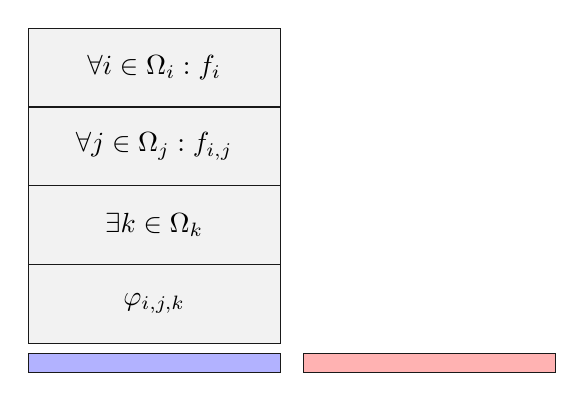
\begin{tikzpicture}[nodes={draw=black!90, fill=gray!10,
        minimum height=\h,
        minimum width=\w,
        },
    row sep=0.3cm,column sep=0.5cm]
        \base{0}{blue}
        \stack{0}{3}{$\forall i\in \Omega_i : f_i$}
        \stack{0}{2}{$\forall j \in \Omega_j : f_{i, j}$}
        \stack{0}{1}{$\exists k \in \Omega_k$}
        \stack{0}{0}{$\varphi_{i, j, k}$}
        %\arrow{0}
        \base{1}{red}
        %\stack{1}{3}{$\forall i\in \Omega_i$}
        %\stack{1}{2}{$\forall j \in \Omega_j$}
        %\stack{1}{1}{$\exists k \in \Omega_k$}
        %\stack{1}{0}{$\Phi_{i, j, k}$}
        %\arrow{1}
    \end{tikzpicture}
    \bigskip\break
    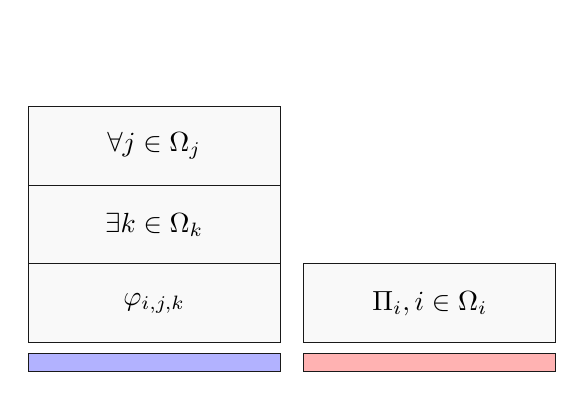
\begin{tikzpicture}[nodes={draw=black!90, fill=gray!5,
        minimum height=\h,
        minimum width=\w,
        },
    row sep=0.3cm,column sep=0.5cm]
        \base{0}{blue}
        \xtack{0}{3}{$\forall i\in \Omega_i$}
        \stack{0}{2}{$\forall j \in \Omega_j$}
        \stack{0}{1}{$\exists k \in \Omega_k$}
        \stack{0}{0}{$\varphi_{i, j, k}$}
        %\arrow{0}
        \base{1}{red}
        \stack{1}{0}{$\Pi_{i}, i\in \Omega_i$}
        %\stack{1}{2}{$\forall j \in \Omega_j$}
        %\stack{1}{1}{$\exists k \in \Omega_k$}
        %\stack{1}{0}{$\Phi_{i, j, k}$}
        %\arrow{1}
    \end{tikzpicture}
    %%
    \label{fig:compiler-stack}
    \caption{O processo de análise dos quantificadores.}
\end{figure}